\chapter{Three Current-Mirror OTA simulation to achieve desired specifications}
\label{ch:chap1}

\section{Introduction}
Operational Transconductance Amplifiers (OTAs) play a crucial role in analog circuit design, particularly in applications such as filters, analog-to-digital converters, and signal processing circuits. Among various OTA architectures, the Three Current-Mirror OTA offers a balance between gain, bandwidth, and power consumption, making it suitable for low-voltage, high-performance applications.

A basic differential amplifier, as shown in Figure~\ref{fig:diff_amp}, consists of a differential pair biased by a simple current mirror and an active PMOS load. While this configuration provides fundamental amplification capabilities, its performance is limited in terms of gain and bandwidth. To enhance performance, a modified architecture known as the Three Current-Mirror OTA is implemented, as depicted in Figure~\ref{fig:three_mirror}. This configuration incorporates self-biased loads and additional current mirrors to improve gain and bandwidth efficiency.

The primary objective of this project is to design and simulate a Three Current-Mirror OTA while maximizing the Gain Bandwidth Product (GBW). The design adheres to specific performance constraints, including a minimum open-loop gain of 40 dB, unity gain frequency above 20 MHz, and a phase margin greater than 45$^\circ$. Additionally, power consumption is limited to 1000 $\mu$W to ensure energy efficiency.

The remainder of this report details the design methodology, including transistor sizing calculations and simulation results. Performance metrics such as DC gain, unity gain bandwidth, and phase margin are analyzed, followed by a comparison with theoretical expectations. The final section provides a discussion on design trade-offs and potential improvements for future implementations.

\begin{figure}[h]
\centering
\begin{subfigure}[b]{0.45\textwidth}
\centering
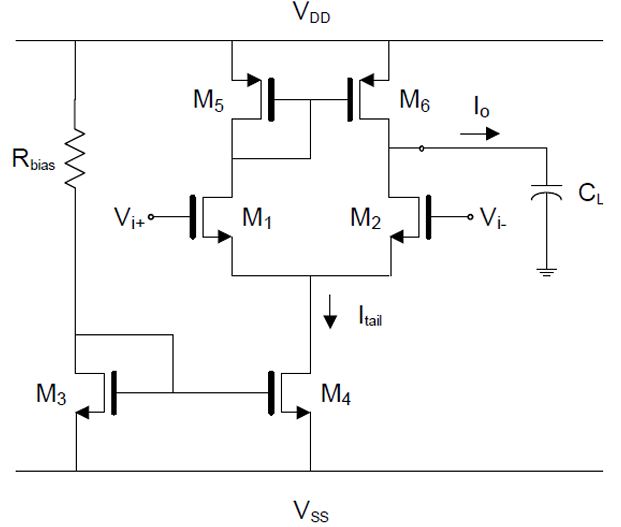
\includegraphics[width=\textwidth]{diff_amp.png}
\caption{Simple Differential Amplifier used as a single-stage basic OTA (5-transistor OTA).}
\label{fig:diff_amp}
\end{subfigure}
\hfill
\begin{subfigure}[b]{0.45\textwidth}
\centering
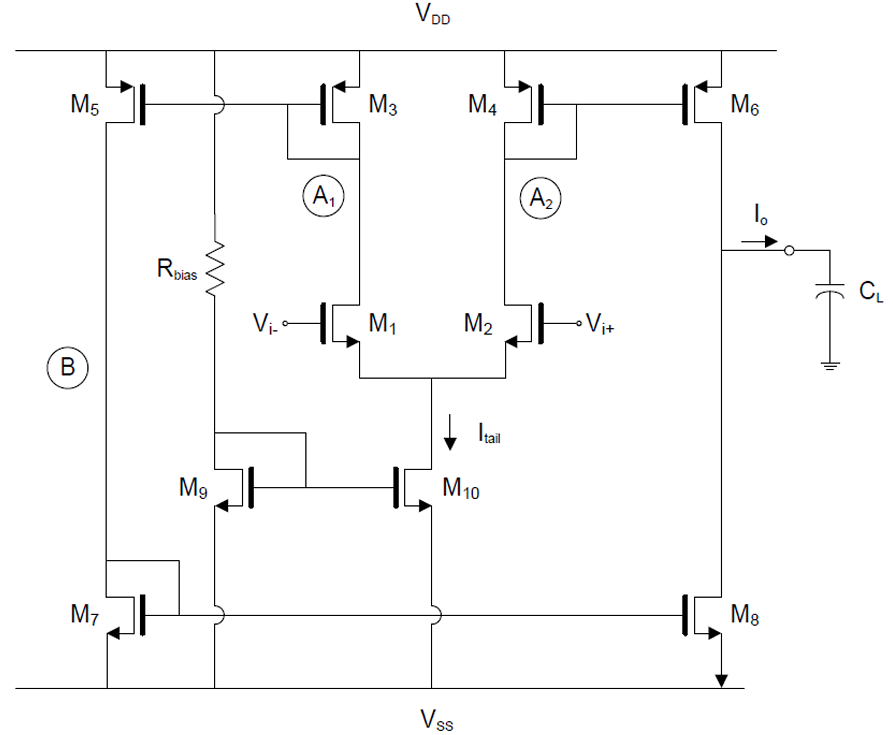
\includegraphics[width=\textwidth]{three_mirror.png}
\caption{Two-stage single-ended symmetric OTA (Three Current-Mirror OTA).}
\label{fig:three_mirror}
\end{subfigure}
\caption{Comparison of different OTA architectures.}
\end{figure}






\section{Single Stage OTA}
\begin{figure}[h]
    \centering
    \includegraphics[width=0.7\textwidth]{}
    \caption{Schematic of the single-stage amplifier circuit.}
\end{figure}

\section{Design Methodology and Details of the Calculation and Device Sizes}

\subsection{Project Performance Specifications}
\captionsetup{justification=centerlast} % Center the caption
\begin{center}
    \begin{table}[h]
    \centering
    \renewcommand{\arraystretch}{1.2}
    \caption{Required Project Performance Specifications}
    \begin{tabular}{l l}
        \toprule
        \textbf{Parameter} & \textbf{Project Specification} \\
        \midrule
        Technology [Min. length of transistors ($L_{min}$)] & 45 nm CMOS \\
        Supply voltage $V_{DD}$ & 1 V \\
        GND & 0 V \\
        Output load capacitance $C_L$ & 20 pF \\
        Nominal input common-mode voltage $V_{DD}/2$ & 0.5 V \\
        Reference current $I_{REF}$ & 2 $\mu$A (change accordingly) \\
        Overall DC power consumption $P_{total}$ & $\leq$ 1000 $\mu$W \\
        \midrule
        Open-loop low-frequency (DC) gain $A_{DC}$ & $\geq$ 100 (40 dB) (maximize) \\
        Unity gain frequency $f_U$ & $\geq$ 20 MHz (maximize) \\
        Phase Margin $PM$ & $>$ 45$^\circ$ \\
        Slew rate (both open-loop and closed-loop) $SR$ & $>$ 10 V/$\mu$s \\
        \bottomrule
    \end{tabular}
\end{table}
\end{center}
 I calculated the following parameters with the help of given constraints:
\subsubsection{Assumptions}
\begin{itemize}
    \item I$_{\text{CMR}-}$ = 0.5V (minimum V$_{CM}$ to keep NMOS and tail in saturation).
    \item I$_{\text{CMR}+}$ = 0.9V (maximum V$_{CM}$ before PMOS or output limits are exceeded).
\end{itemize}

\subsection{Transistor Parameters from Cadence Simulation}
The following parameters are obtained from Cadence simulation for NMOS and PMOS design
with channel length $L = 1\mu$m (to minimize the channel length modulation) and width $W = 10\mu$m
for both NMOS and PMOS transistors. The supply voltage is $V_{DD} = 1$V, and the bias current is
$I_o = 10\mu$A.

\subsubsection{NMOS Parameters}
\begin{itemize}
    \item Effective Beta ($\beta_{\text{eff, NMOS}}$): 3.40095 mA/V$^2$ (approximated as 3 mA/V$^2$)
    \item Threshold Voltage ($V_{\text{th, NMOS}}$): 397.501 mV (approximated as 0.4 V)
\end{itemize}

\subsubsection{PMOS Parameters}
\begin{itemize}
    \item Effective Beta ($\beta_{\text{eff, PMOS}}$): 2.86778 mA/V$^2$ (approximated as 3 mA/V$^2$)
    \item Threshold Voltage ($V_{\text{th, PMOS}}$): -334.416 mV (approximated as -0.3 V)
\end{itemize}

\subsection{Calculation of $\mu C_{ox}$ for NMOS and PMOS}
The effective beta ($\beta_{\text{eff}}$) is related to the process transconductance parameter $\mu C_{ox}$ by the equation:
\begin{equation}
    \beta_{\text{eff}} = \mu C_{ox} \frac{W}{L}
\end{equation}
where $W = 10\mu$m, $L = 1\mu$m, and $\frac{W}{L} = 10$. Using the approximated effective beta values from Cadence simulation:

\subsubsection{NMOS $\mu_n C_{ox}$ Calculation}
\begin{align*}
    \beta_{\text{eff, NMOS}} &\approx 3 \text{ mA/V}^2 \\
    \mu_n C_{ox} &= \frac{\beta_{\text{eff, NMOS}}}{\frac{W}{L}} \\
    \mu_n C_{ox} &= \frac{3 \text{ mA/V}^2}{10} \\
    \mu_n C_{ox} &= 0.3 \text{ mA/V}^2
\end{align*}

\subsubsection{PMOS $\mu_p C_{ox}$ Calculation}
\begin{align*}
    \beta_{\text{eff, PMOS}} &\approx 3 \text{ mA/V}^2 \\
    \mu_p C_{ox} &= \frac{\beta_{\text{eff, PMOS}}}{\frac{W}{L}} \\
    \mu_p C_{ox} &= \frac{3 \text{ mA/V}^2}{10} \\
    \mu_p C_{ox} &= 0.3 \text{ mA/V}^2
\end{align*}

\subsection{Calculations}
\begin{itemize}
    \item All MOSFETs should be in the saturation region.
    \item $I_o \rightarrow$ Slew rate – Derivation of $I_o$:
\end{itemize}

The relationship between charge and current is given by:
\begin{equation}
    \frac{dq}{dt} = I = C \frac{dv}{dt}
\end{equation}
where the Slew Rate (SR) is defined as:
\begin{equation}
    SR = \frac{dv}{dt}
\end{equation}

Rearranging for $I_o$:
\begin{equation}
    SR = \frac{I_o}{C_L}
\end{equation}

(Slew rate as a function of output current and load capacitance)

Solving for $I_o$ with $SR = 10$ V/$\mu$s and $C_L = 2$ pF:
\begin{align*}
    I_o &= SR \cdot C_L \\
        &= 10 \text{ V}/\mu\text{s} \times 2\text{ pF} \\
        &= 20 \mu\text{A}
\end{align*}

\begin{itemize}
    \item $M_5, M_6 \rightarrow ICMR^+ = 0.9V$
\end{itemize}

%\subsection{Calculation of $V_{DS}$ and $V_1$}
\begin{align*}
    V_{DS} &\geq V_{GS} - V_{th} \\
    V_D &\geq V_{GS} - V_{th} \\
    V_1 &\geq V_{in} - V_{th} \\
    V_1 &\geq 0.9 - 0.4 \\
    V_1 &\geq 0.5 \\
    \Rightarrow V_1 &= 0.5V \\
    V_{DS} &= V_{DD} - V_1 \\
    V_{DS} &= 1V - 0.5V \\
    V_{DS} &= 0.5V \\
    I_o &= 10\mu A
\end{align*}

\subsection{Calculation of $W/L$ Ratio for $M_5$ and $M_6$}

The drain current $I_D$ in the saturation region is given by:
\begin{equation}
    I_D = \frac{1}{2} \mu_n C_{ox} \frac{W}{L} (V_{GS} - V_{th})^2
\end{equation}
where:
\begin{itemize}
    \item $\mu_n C_{ox} = 0.3 \text{ mA}/\text{V}^2$
    \item $I_D = I_o = 10 \mu A = 0.01 \text{ mA}$
    \item $V_{DS} = V_{GS} = 0.5V$ (since Gate and Drain are shorted)
    \item $V_{th} \approx 0.4V$
    \item $L = 1 \mu m$
\end{itemize}

\subsubsection{Derivation of $W/L$}

Rearrange the equation to solve for $\frac{W}{L}$:
\begin{equation}
    \frac{W}{L} = \frac{2 I_D}{\mu_n C_{ox} (V_{GS} - V_{th})^2}
\end{equation}

Substitute the known values:
\begin{align*}
    I_D &= 0.01 \text{ mA} \\
    \mu_n C_{ox} &= 0.3 \text{ mA}/\text{V}^2 \\
    V_{GS} - V_{th} &= 0.5V - 0.3V = 0.2V \\
    (V_{GS} - V_{th})^2 &= (0.2V)^2 = 0.04V^2 \\
    \mu_n C_{ox} \times (V_{GS} - V_{th})^2 &= 0.3 \text{ mA}/\text{V}^2 \times 0.04 \text{ V}^2 = 0.012 \text{ mA}
\end{align*}

Now calculate:
\begin{equation}
    \frac{W}{L} = \frac{2 \times 0.01 \text{ mA}}{0.012 \text{ mA}} \approx 1.667 \Rightarrow \frac{W}{L} \approx 2
\end{equation}

\subsection{Open-Loop Gain Derivation for OTA}
The open-loop gain $A_0$ of the OTA is defined as the ratio of the output voltage to the input voltage:
\begin{equation}
    A_0 = \frac{V_{\text{out}}}{V_{\text{in}}}
\end{equation}

This can be expressed as:
\begin{equation}
    \frac{V_{\text{out}}}{V_{\text{in}}} = (r_{op} \parallel r_{on}) \cdot g_{m,n} \Delta V_{\text{in}} \cdot \frac{1}{\Delta V_{\text{in}}}
\end{equation}

Since $\Delta V_{\text{in}}$ cancels out, the gain simplifies to:
\begin{equation}
    A_0 = (r_{op} \parallel r_{on}) \cdot g_{m,n}
\end{equation}
where:
\begin{itemize}
    \item $r_{op}$: Output resistance of the M6 (PMOS transistor),
    \item $r_{on}$: Output resistance of the M2 (NMOS transistor),
\end{itemize}

\subsection{Gain-Bandwidth Product (GB) Derivation}
The Gain-Bandwidth Product (GB) is defined as the product of the DC gain $A_0$ and the unity-gain bandwidth $f_{GB}$:
\begin{equation}
    GB = A_0 \cdot f_{GB}
\end{equation}

The unity-gain bandwidth $f_{GB}$ for the OTA can be approximated as:
\begin{equation}
    f_{GB} = \frac{1}{(r_{op} \parallel r_{on}) \cdot 2\pi C_L}
\end{equation}
where:
\begin{itemize}
    \item $g_{m1,2}$: Transconductance of the input NMOS transistors (M1, M2),
    \item $C_L$: Load capacitance at the output node.
\end{itemize}

Substituting the expression for $A_0$:
\begin{equation}
    A_0 = (r_{op} \parallel r_{on}) \cdot g_{m1,2}
\end{equation}

The GB product becomes:
\begin{equation}
    GB = \left[ (r_{op} \parallel r_{on}) \cdot g_{m1,2} \right] \cdot \frac{1}{(r_{op} \parallel r_{on}) \cdot 2\pi C_L}
\end{equation}

Simplifying, the GB can be expressed as:
\begin{equation}
    GB = \frac{g_{m1,2}}{2\pi C_L}
\end{equation}

Given $GB = 20 \text{ MHz}$ and $C_L = 2 \text{ pF}$, we can solve for $g_{m1,2}$:
\begin{equation}
    GB = \frac{g_{m1,2}}{2\pi C_L}
\end{equation}

\begin{equation}
    g_{m1,2} = GB \cdot 2\pi C_L
\end{equation}

Substituting the values ($GB = 20 \times 10^6 \text{ Hz}$, $C_L = 2 \times 10^{-12} \text{ F}$):
\begin{equation}
    g_{m1,2} \approx 40 \times 2 \times \pi \times 10^{-6} \approx 251.3 \times 10^{-6} \text{ S}
\end{equation}

\begin{equation}
    g_{m1,2} \approx 251.33 \mu\text{S}
\end{equation}

\subsection{Calculation of $W/L$ Ratios for M1 and M2}
The drain current $I_D$ for a MOSFET in saturation is given by:
\begin{equation}
    I_D = \frac{1}{2} \mu C_{ox} \frac{W}{L} (V_{GS} - V_t)^2
\end{equation}

The transconductance $g_m$ is the derivative of $I_D$ with respect to $V_{GS}$:
\begin{equation}
    g_m = \frac{\partial I_D}{\partial V_{GS}} = \mu C_{ox} \frac{W}{L}
\end{equation}

Squaring both sides and relating to $I_D$:
\begin{equation}
    g_m^2 = 2 \mu C_{ox} \frac{W}{L} (V_{GS} - V_t) I_D
\end{equation}

Solving for $\frac{W}{L}$:
\begin{equation}
    \frac{W}{L} = \frac{g_m^2}{2 \mu C_{ox} I_D}
\end{equation}

Given:
\begin{itemize}
    \item $\mu C_{ox} = 0.3 \text{ mA/V}^2$ (for NMOS),
    \item $I_D = I_o = 10 \mu A = 0.01 \text{ mA}$,
    \item $g_{m1,2} \approx 251.3 \mu S = 0.2513 \text{ mS}$ (from GB derivation),
\end{itemize}

Substitute into the $W/L$ equation:
\begin{equation}
    \frac{W}{L} = \frac{(0.2513 \times 10^{-3})^2}{2 \cdot (0.3 \times 10^{-3}) \cdot (0.01 \times 10^{-3})}
\end{equation}

Calculate step-by-step:
\begin{equation}
    g_m^2 = (0.2513 \times 10^{-3})^2 = 6.3147 \times 10^{-8} \text{ S}^2
\end{equation}
\begin{equation}
    2 \mu C_{ox} I_D = 2 \cdot (0.3 \times 10^{-3}) \cdot (0.01 \times 10^{-3}) = 6 \times 10^{-9} \text{ A/V}^2
\end{equation}

Thus,
\begin{equation}
    \frac{W}{L} = \frac{6.3147 \times 10^{-8}}{6 \times 10^{-9}} \approx 10.5245
\end{equation}

Therefore, the aspect ratio is:
\begin{equation}
    \frac{W}{L} \approx 10.52 \approx 11
\end{equation}


\subsection{Calculation of $V_{GS}$ for M1}

The drain current $I_D$ for a MOSFET in saturation is given by:
\begin{equation}
    I_D = \frac{1}{2} \mu C_{ox} \frac{W}{L} (V_{GS} - V_{TH})^2
\end{equation}

Given:
\begin{itemize}
    \item $I_D = I_o = 10 \mu A = 0.01 \times 10^{-3} A$,
    \item $\mu C_{ox} = 0.3 \text{ mA/V}^2 = 0.3 \times 10^{-3} \text{ A/V}^2$,
    \item $\frac{W}{L} = 20$,
    \item $V_{TH} \approx 0.4 \text{ V}$ (threshold voltage).
\end{itemize}

Rearrange the equation to solve for $(V_{GS} - V_{TH})$:
\begin{equation}
    (V_{GS} - V_{TH})^2 = \frac{2I_D}{\mu C_{ox} \frac{W}{L}}
\end{equation}

Substitute the values:
\begin{equation}
    (V_{GS} - V_{TH})^2 = \frac{2 \times (0.01 \times 10^{-3})}{(0.3 \times 10^{-3}) \times 20}
\end{equation}

Calculate step-by-step:
\begin{itemize}
    \item Numerator: $2 \times 0.01 \times 10^{-3} = 0.02 \times 10^{-3} \text{ A}$,
    \item Denominator: $(0.3 \times 10^{-3}) \times 20 = 6 \times 10^{-3} \text{ A/V}^2$.
\end{itemize}

Thus:
\begin{equation}
    (V_{GS} - V_{TH})^2 = \frac{0.02 \times 10^{-3}}{6 \times 10^{-3}} \approx 0.0033 \text{ V}^2
\end{equation}

Solving for $V_{GS} - V_{TH}$:
\begin{equation}
    V_{GS} - V_{TH} = \sqrt{0.0033} \approx 0.0577 \text{ V}
\end{equation}

Therefore, the gate-source voltage is:
\begin{equation}
    V_{GS} = V_{TH} + (V_{GS} - V_{TH}) \approx 0.4 \text{ V} + 0.0577 \text{ V} \approx 0.4577 \text{ V}
\end{equation}

Rounding to two decimal places:
\begin{equation}
    V_{GS} \approx 0.46 \text{ V}
\end{equation}

\subsection{Calculation of $W/L$ for M3 and M4}

Given the constraint $V_{IN} > V_{GS} + V_{DSAT}$, where:
\begin{itemize}
    \item $V_{IN} = V_{ICMR^-} = 0.5 \text{ V}$,
    \item $V_{DSAT} < 0.04 \text{ V}$ (use maximum $V_{DSAT} = 0.04 \text{ V}$ for calculation),
\end{itemize}

Given:
\begin{itemize}
    \item $I_D = 20 \mu A = 0.02 \times 10^{-3} \text{ A}$,
    \item $\mu C_{ox} = 0.3 \text{ mA/V}^2 = 0.3 \times 10^{-3} \text{ A/V}^2$,
    \item $V_{DSAT} < 0.04 \text{ V}$ (use maximum $V_{DSAT} = 0.04 \text{ V}$ for minimum $W/L$).
\end{itemize}

Rearrange for $\frac{W}{L}$:
\begin{equation}
    \frac{W}{L} = \frac{2I_D}{\mu C_{ox} (V_{DSAT})^2}
\end{equation}

Substitute the values:
\begin{equation}
    \frac{W}{L} = \frac{2 \times (0.02 \times 10^{-3})}{(0.3 \times 10^{-3}) \times (0.04)^2}
\end{equation}

Calculate step-by-step:
\begin{itemize}
    \item Numerator: $2 \times 0.02 \times 10^{-3} = 0.04 \times 10^{-3} \text{ A}$,
    \item Denominator: $(0.3 \times 10^{-3}) \times (0.04)^2 = 0.00048 \times 10^{-3} \text{ A/V}^2$.
\end{itemize}

Thus:
\begin{equation}
    \frac{W}{L} = \frac{0.04 \times 10^{-3}}{0.00048 \times 10^{-3}} \approx 83.33
\end{equation}

Rounding to the nearest integer:
\begin{equation}
    \frac{W}{L} \approx 84
\end{equation}

\begin{table}[h]
    \centering
    \renewcommand{\arraystretch}{1.2}
    \begin{tabular}{|l|c|c|c|c|}
        \hline
        \textbf{Parameter} & \textbf{Symbol} & \textbf{Approximated W/L} & \textbf{Chosen W/L} & \textbf{Unit} \\
        \hline
        Chosen Channel Length & $L$ & - & 0.1 & $\mu$m \\
        \hline
        W/L Ratio for $M_1, M_2$ & $W/L_{M_1,M_2}$ & 10.52 & 20 & - \\
        \hline
        W/L Ratio for $M_3, M_4$ & $W/L_{M_3,M_4}$ & 83.33 & 84 & - \\
        \hline
        W/L Ratio for $M_5, M_6$ & $W/L_{M_5,M_6}$ & 1.67 & 2 & - \\
        \hline
        Output Current & $I_o$ & - & 20 & $\mu$A \\
        \hline
        Transconductance & $g_{m1,2}$ & - & 251.33 & $\mu$S \\
        \hline
        Gate-Source Voltage for $M_1$ & $V_{GS}$ & - & 0.46 & V \\
        \hline
        NMOS $\mu C_{ox}$ & $\mu_n C_{ox}$ & - & 0.3 & mA/V$^2$ \\
        \hline
        PMOS $\mu C_{ox}$ & $\mu_p C_{ox}$ & - & 0.3 & mA/V$^2$ \\
        \hline
        NMOS Threshold Voltage & $V_{th,NMOS}$ & - & 0.4 & V \\
        \hline
        PMOS Threshold Voltage & $V_{th,PMOS}$ & - & -0.3 & V \\
        \hline
    \end{tabular}
    \caption{Summary of Calculated Values}
    \label{tab:summary_values}
\end{table}


\section{Simulation results (AC/Transient Simulations showing DC gain, UGBW, PM, and Slew rate)}



\subsection{OpenLoopOTA (Without Feedback)}

\subsubsection{Transient Analysis Setup}

\begin{table}[h]
    \centering
    \caption{Transient Analysis Parameters}
    \begin{tabular}{|c|c|c|}
        \hline
        \textbf{Variable} & \textbf{Symbol} & \textbf{Value} \\
        \hline
        Vin+ Delay Time & vinp delay & 1 $\mu$s \\
        Vin+ Zero Value & vinp zero & 1 V \\
        Vin+ One Value & vinp one & 0 V \\
        Vin+ Period of Waveform & vinp period & 10 $\mu$s \\
        Vin+ Rise Time & vinp rise & 50 ns \\
        Vin+ Fall Time & vinp fall & 50 ns \\
        Vin- Delay Time & vinn delay & 1 $\mu$s \\
        Vin- Zero Value & vinn zero & 0 V \\
        Vin- One Value & vinn one & 1 V \\
        Vin- Period of Waveform & vinn period & 10 $\mu$s \\
        Vin- Rise Time & vinn rise & 50 ns \\
        Vin- Fall Time & vinn fall & 50 ns \\
        \hline
    \end{tabular}
\end{table}

\subsubsection{Slew Rate Analysis}
The slew rate (SR) is calculated based on the rising edge, representing the maximum rate of change of the output voltage ($V_{OUT}$):

\begin{equation}
    SR = \frac{\Delta V_{OUT}}{\Delta t}
\end{equation}

From the transient response, $V_{OUT}$ transitions from 100 mV to 900 mV over 11.0399 $\mu$s to 11.161 $\mu$s:

\begin{equation}
    SR = \frac{900 \times 10^{-3} - 100 \times 10^{-3}}{11.161 \times 10^{-6} - 11.0399 \times 10^{-6}}
\end{equation}

\begin{equation}
    SR = \frac{800 \times 10^{-3}}{0.1211 \times 10^{-6}}
\end{equation}

\begin{equation}
    SR \approx 6.6061 \text{ V/} \mu s
\end{equation}

\subsubsection{AC Analysis Setup}
For the AC analysis, a 500 mV DC voltage with a 1 V AC signal, incorporating two signals with 0$^\circ$ and 180$^\circ$ phase shifts, was applied.

\subsubsection{AC Analysis Results}
The AC analysis results are derived from the frequency response plot:

\begin{itemize}
    \item \textbf{DC Gain}: Approximately 22.3856 dB at 1 nHz, below the specification of $\geq$ 40 dB.
    \item \textbf{Unity Gain Bandwidth (UGBW)}: Approximately 1.12173 MHz, below the specification of $\geq$ 20 MHz.
    \item \textbf{Phase Margin (PM)}: At 1.12173 MHz, the phase is $-85.6714^\circ$, giving:
    \begin{equation}
        PM = 180^\circ - 85.6714^\circ \approx 94.3286^\circ
    \end{equation}
    This exceeds the specification of $>$ 45$^\circ$.
\end{itemize}

\begin{table}[h]
    \centering
    \caption{Comparison of Open Loop Results with Design Specifications}
    \begin{tabular}{|c|c|c|c|}
        \hline
        \textbf{Parameter} & \textbf{Design Specification} & \textbf{Obtained Value} & \textbf{Unit} \\
        \hline
        Open-loop DC Gain & $\geq$100 (40 dB) & 22.3856 & dB \\
        Unity Gain Frequency & $\geq$20 MHz & 1.12173 & MHz \\
        Phase Margin & $>$45$^\circ$ & 94.3286$^\circ$ & $^\circ$ \\
        Slew Rate & $>$10 V/$\mu$s & 6.6061 & V/$\mu$s \\
        \hline
    \end{tabular}
\end{table}


\subsection{Closed Loop OTA (With Unity Gain Feedback)}

\subsubsection{Transient Analysis Setup}

\begin{table}[h]
    \centering
    \caption{Transient Analysis Parameters}
    \begin{tabular}{|c|c|c|}
        \hline
        \textbf{Variable} & \textbf{Symbol} & \textbf{Value} \\
        \hline
        Vin+ Delay Time & vinp delay & 1 $\mu$s \\
        Vin+ Zero Value & vinp zero & 1 V \\
        Vin+ One Value & vinp one & 0 V \\
        Vin+ Period of Waveform & vinp period & 10 $\mu$s \\
        Vin+ Rise Time & vinp rise & 50 ns \\
        Vin+ Fall Time & vinp fall & 50 ns \\
        \hline
    \end{tabular}
\end{table}

\subsubsection{Pulse Input Configuration}
The transient response is driven by a pulse input with the following parameters:

\begin{equation}
    SR = \frac{\Delta V_{OUT}}{\Delta t}
\end{equation}

From the transient response, $V_{OUT}$ transitions from 158.34011 mV to 777.86979 mV over 1.0375 $\mu$s to 1.1302 $\mu$s:

\begin{equation}
    SR = \frac{777.86979 \times 10^{-3} - 158.34011 \times 10^{-3}}{1.13024 \times 10^{-6} - 1.0375 \times 10^{-6}}
\end{equation}

\begin{equation}
    SR = \frac{619.52968 \times 10^{-3}}{0.09274 \times 10^{-6}}
\end{equation}

\begin{equation}
    SR \approx 6.6803 \text{ V/} \mu s
\end{equation}

\subsubsection{AC Analysis Setup}
For the AC analysis, a 500 mV DC voltage with a 1 V AC signal was applied to the $V_{INP}$ terminal.

\section{Two-Stage OTA}

\subsection{Introduction to Two-Stage OTA Design}
An enhancement to the differential amplifier involves the incorporation of self-biased loads. This configuration is referred to as a two-stage single-ended symmetric OTA, commonly known as a three current-mirror OTA. The input stage comprises a differential pair, while the sub-circuits consisting of $M_1, M_3$ and $M_2, M_4$ function as self-biased inverters. The transistors $M_3, M_5$, $M_4, M_6$, $M_7, M_8$, and $M_9, M_{10}$ are configured as simple current mirrors.

In the design of this symmetric OTA, the transistors are symmetrically matched such that:
\begin{align*}
    M_1 &= M_2, \\
    M_3 &= M_4, \\
    M_5 &= M_6, \\
    M_7 &= M_8.
\end{align*}

This symmetry reduces the number of adjustable parameters to four transistor sizes and the tail current, simplifying the design process while maintaining balanced performance.

\begin{figure}[h]
    \centering
    \includegraphics[width=0.7\textwidth]{} % Add the correct path to the image
    \caption{Single Stage and Two-Stage OTAs}
    \label{fig:single_two_stage_ota}
\end{figure}

\subsection{Device Sizing Calculations}
\begin{figure}[h]
    \centering
    \includegraphics[width=0.7\textwidth]{} % Add the correct path to the image
    \caption{Two-stage single-ended symmetric OTA (Three current-mirror OTA)}
    \label{fig:two_stage_ota}
\end{figure}

\subsection{Transition from Single-Stage to Two-Stage OTA Design}
Having completed the calculations for the single-stage OTA, the next step involves determining the $W/L$ ratios for the two-stage single-ended symmetric OTA. To facilitate this transition, mappings from the single-stage to the two-stage design can be established based on the previously calculated ratios. 

Specifically, the $W/L$ ratio of $20$, determined for $M_1$ and $M_2$ in the single-stage OTA, can be directly applied to $M_1$ and $M_2$ in the two-stage configuration, maintaining the input differential pair symmetry. Similarly, the $W/L$ ratio of $2$, originally calculated for $M_5$ and $M_6$ (related to $M_3$ and $M_4$ in the single-stage design), can be adopted for $M_3$ and $M_4$ in the two-stage OTA. For $M_9$ and $M_{10}$, which correspond to $M_3$ and $M_4$ in the single-stage case, the $W/L$ ratio of $84$ can be applied.

Further, considering the current distribution across each branch, the $W/L$ ratios for the remaining MOSFETs can be derived. For instance, the $W/L$ ratio for $M_5$ and $M_6$ can be set to twice that of $M_3$ and $M_4$, yielding:
\begin{equation*}
    2 \times 2 = 4.
\end{equation*}
Likewise, the $W/L$ ratio of $84$ can be retained for $M_7$ and $M_8$ in the two-stage configuration, ensuring consistency in the current mirror design.

\subsection{Summary of W/L Ratios for Two-Stage OTA}
\begin{table}[h]
    \centering
    \caption{Summary of W/L Ratios for Two-Stage OTA}
    \begin{tabular}{|c|c|c|}
        \hline
        Transistor Pair & W/L Ratio & Width (W) [\textmu m] \\
        \hline
        $M_1, M_2$ (Differential Pair) & 20 & 2.4 \\
        $M_3, M_4$ (Self-Biased Inverters) & 2 & 0.24 \\
        $M_5, M_6$ (Current Mirror) & 4 & 0.48 \\
        $M_7, M_8$ (Current Mirror) & 84 & 10 \\
        $M_9, M_{10}$ (Current Mirror) & 84 & 10 \\
        \hline
    \end{tabular}
\end{table}

\subsection{Simulation Results}
\subsubsection{Open Loop Case (Without Feedback)}
\paragraph{Transient Analysis}
\begin{table}[h]
    \centering
    \caption{Transient Analysis Parameters}
    \begin{tabular}{|c|c|}
        \hline
        Variable & Value \\
        \hline
        $V_{in+}$ Delay Time & 1 \textmu s \\
        $V_{in+}$ Zero Value & 1 V \\
        $V_{in+}$ One Value & 0 V \\
        $V_{in+}$ Period & 10 \textmu s \\
        $V_{in+}$ Rise Time & 50 ns \\
        $V_{in+}$ Fall Time & 50 ns \\
        \hline
    \end{tabular}
\end{table}

\paragraph{Slew Rate Analysis}
\begin{equation*}
    SR = \frac{\Delta V_{OUT}}{\Delta t}
\end{equation*}
\begin{equation*}
    SR = \frac{900 \times 10^{-3} - 100 \times 10^{-3}}{5.18482 \times 10^{-6} - 5.08923 \times 10^{-6}} = \frac{800 \times 10^{-3}}{0.09559 \times 10^{-6}} \approx 8.3691 V/\textmu s
\end{equation*}

\paragraph{AC Analysis}
DC Gain: $21.1052$ dB at $1$ nHz.\\
Unity Gain Bandwidth (UGBW): $10.2355$ MHz.\\
Phase Margin (PM): $85.3505^{\circ}$ at $10.2355$ MHz.

\subsubsection{Closed Loop Case (With Unity Feedback)}
\paragraph{Slew Rate Analysis}
\begin{equation*}
    SR = \frac{809.658 \times 10^{-3} - 275.849 \times 10^{-3}}{14.6207 \times 10^{-6} - 14.5777 \times 10^{-6}} = \frac{533.809 \times 10^{-3}}{0.043 \times 10^{-6}} \approx 12.4142 V/\textmu s
\end{equation*}


\section{ A(table of) comparison between design/simulation results and a brief explanation}



















    \begin{figure}[h]
        \centering
           \includegraphics[width=0.35\textwidth]{}
        \caption{}
        \label{fig: }
    \end{figure}

\endinput